\documentclass{article}

% Formatting
\usepackage[utf8]{inputenc}
\usepackage[margin=1in]{geometry}
\usepackage[titletoc,title]{appendix}
\usepackage{listings}
\usepackage{xcolor}
\usepackage{titling}
\usepackage{indentfirst}

\lstset{%
  language=Python,
  basicstyle   = \ttfamily,
  keywordstyle =    \color{magenta},
  keywordstyle = [2]\color{orange},
  commentstyle =    \color{gray}\itshape,
  stringstyle  =    \color{cyan},
  numbers      = left,
  frame        = single,
  framesep     = 2pt,
  aboveskip    = 1ex,
  showstringspaces=false,
  literate=%
  {\%}{{{\color{orange}\%}}}1
  {!=}{{{\color{orange}!=}}}1
}

\usepackage{amsmath,amsfonts,amssymb,mathtools}
\usepackage{graphicx,float}
\usepackage[ruled,vlined]{algorithm2e}
\usepackage{algorithmic}
\usepackage{caption}
\usepackage{subcaption}
\usepackage{float}
\usepackage{biblatex}
\addbibresource{references.bib}

\pretitle{
  \begin{center}
  \LARGE
  
\includegraphics[width=6cm]{logo}\\[\bigskipamount]
  \end{center}
}


\begin{document}

%\maketitle
\begin{titlepage} 
	\newcommand{\HRule}{\rule{\linewidth}{0.5mm}} % Defines a new command for horizontal lines, change thickness here
	
	\center % Centre everything on the page
	
	%------------------------------------------------
	%	Headings
	%------------------------------------------------
	
	%\textsc{\LARGE Sorbonne université}\\ % Main heading such as the name of your university/college
	
\includegraphics[width=0.5\textwidth]{logo.png}\\[1cm] 
	\textsc{\Large Complex: 4I900}\\[0.5cm] % Major heading such as course name
	
	%------------------------------------------------
	%	Title
	%------------------------------------------------
	
	\HRule\\[0.4cm]
	
	{\huge\bfseries Rapport du projet : test primalité}\\[0.4cm] % Title of your document
	
	\HRule\\[1.5cm]
	
	%------------------------------------------------
	%	Author(s)
	%------------------------------------------------
	
	\begin{minipage}{0.4\textwidth}
		\begin{flushleft}
			\large
			\textit{Binôme}\\
			Mounib \textsc{Benimam}\\ % Your name
			Guillaume \textsc{Magniadas}\\
		\end{flushleft}
	\end{minipage}
	~
	\begin{minipage}{0.4\textwidth}
		\begin{flushright}
			\large
			\textit{chargé de Td}\\
			Florette \textsc{Martinez} % Supervisor's name
		\end{flushright}
	\end{minipage}
	
	
	\vfill\vfill\vfill % Position the date 3/4 down the remaining page
	
	{\large\today} 
	
	
	\vfill 
	
\end{titlepage}

\begin{abstract}

En 1801, C. F. Gauss écrivait dans \emph{Disquisitiones Arithmeticae que distinguer nombres
premiers et nombres composés, et décomposer ces derniers en facteurs premiers, est un des
problèmes les plus importants et les plus utiles en arithmétique}. Le but de ce projet est de
présenter certaines méthodes utilisées pour tester la primalité d’un nombre entier. \\

\indent Le problème de primalité est le suivant : \\
\indent \indent \textbf{Entrée} : un entier $N \in \mathbb{N}^{\star}$ \\
\indent \indent \textbf{Question} : N est-il premier ? \\

\noindent Nous allons implanter un test de primalité naiif déterministe dont la complexité est exponentielle. Ensuite, nous allons implanter deux tests probabilistes de primalité efficaces mais qui
se trompent de temps en temps lorsque N est premier. Ainsi, si le test probabiliste retourne
premier alors l’entier est premier avec une certaine probabilité. En revanche, si N est composé
alors le test probabiliste retourne toujours composé.
\end{abstract}

\section{Arithmitique dans $\mathbb{Z}/n\mathbb{Z}$}
Dans cette partie nous allons poser les fonctions de base pour ce qui suit
\subsection{Calcule PGCD}

nous cherchons le dernier reste non nul
\begin{lstlisting}[language=Python, caption=Implémentation de l'algorithme d'euclide]
def my_gcd(a, b):
    """
    int*int -> int
    """
    a, b = max(a, b), min(a, b)
    while b != 0:
        tempo = b
        b = a % b
        a = tempo
    return a
\end{lstlisting}

si nous voulons uniquement le PGCD, l'algorithme simplifié d'euclide est plus rapide et suffisant. mais pour avoir les coefficients de Bezout cela necessiet une implementation complète de l'algorithme d'euclide dit etendu.

\begin{lstlisting}[language=Python, caption=Implémentation de l'algorithme d'Euclide étendu.]
def my_gcd_etendu(a, b):
    """
    int*int-> int*int*int
    """
    a, b = max(a, b), min(a, b)
    u = np.array([a, 1, 0])
    v = np.array([b, 0, 1])

    while(v[0] != 0):
        q = u[0]//v[0]
        temp = v
        v = u - q*v
        u = temp
    return tuple(map(int, u))
\end{lstlisting}

Une des opérations les plus importantes en l'arithmétique modulaire est l'inverse $a^{-1} \in \mathbb{Z}/n\mathbb{Z}$ tel que  $aa^{-1} \equiv 1[n]$, un tel élèment existe ssi a, n sont premier entre eux :
\begin{equation}
    \forall n \forall a, \quad PGCD(a, n)=1 \iff \exists b \in \mathbb{Z}/n\mathbb{Z}, ab \equiv 1[n]
\end{equation}

et particulierement si n est premier un inverse existe toujours et $\mathbb{Z}/n\mathbb{Z}$ est alors un corps.
\begin{equation}
    \forall n, \forall (a<n), \quad \mathit{estPremier}(n) \implies (\mathit{PGCD}(n, a)=1).  
\end{equation}

\begin{lstlisting}[language=Python, caption=Implementation de l'inverse modulaire]
def my_inverse(a, N):
    """int*int->int
    retourner inverse de a modulo N
    """
    # tester tout les nombres
    for b in range(N):
        if(((a*b) % N) == 1):
            return b
    # si on trouve pas d'inverse
    print(f"{a} n'a pas d'inverse modulo {N}")
\end{lstlisting}

\begin{lstlisting}[language=Python, caption=Implementation de l'inverse modulaire Bézout]
def my_inverse_bezout(a, N):
    """ inverse en utilisant euclide_etendu"""
    u0, u1, u2 = my_gcd_etendu(a, N)
    if(u0 == 1):
        return u2 if a<N else u1
    # si on trouve pas d'inverse
    print(f"{a} n'a pas d'inverse modulo {N}")
\end{lstlisting}


\subsubsection{Comparaison en temps}

\begin{minipage}{0.5\textwidth}
    \begin{figure}[H]
        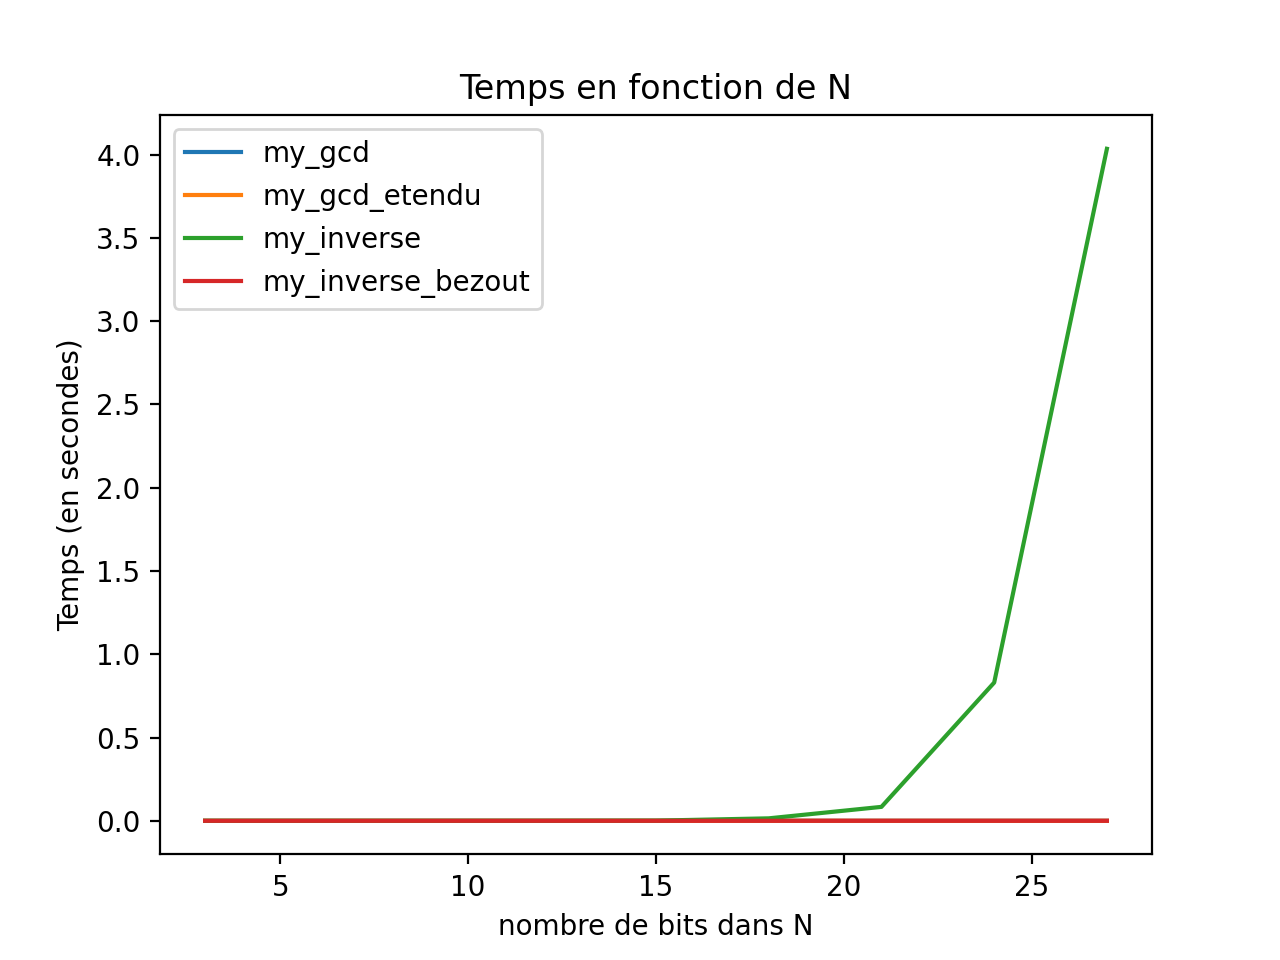
\includegraphics[scale=0.5]{inverse_gcd.png}
        \caption{Comparaison entre les fonctions my\_gcd, my\_gcd\_etendu et my\_inverse}
        \label{rot1}
    \end{figure}
\end{minipage}
\hspace{2ex} 
\begin{minipage}{0.5\textwidth}
    \begin{figure}[H]
        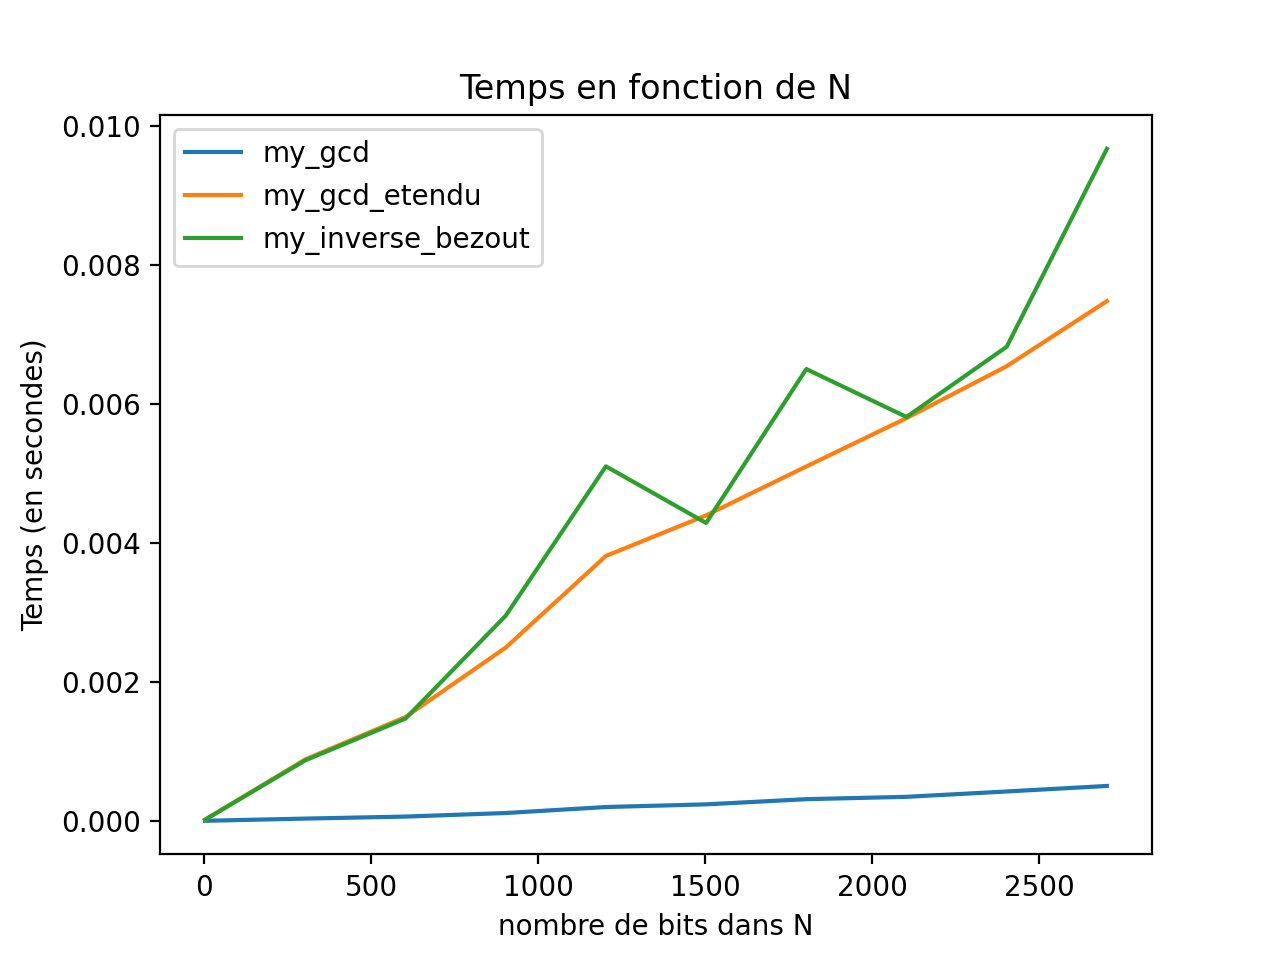
\includegraphics[scale=0.5]{gcd_gcdetendu.png}
        \caption{Comparaison entre les fonctions my\_gcd, my\_gcd\_etendu et my\_inverse}
        \label{rot2}
    \end{figure}
\end{minipage}\\[0.5cm]


On peut observer sur ces courbes que la complexité de my\_gcd et de my\_gcd\_etendu semble être polynomial au nombres de bits tendis que my\_inverse exponentiel au nombre de bits. 

\subsection{my\_expo\_mod}

Implementation de l'algorithme d'exponentiation binaire rapide, complexité en
\begin{lstlisting}[language=Python, caption=my\_expo\_mod]
def my_expo_mod(g, n, N):
    """
    int*int*int -> int
    return (g^n) % N
    """
    h = 1

    if n < 0:
        # puissance negative
        gcd, _, v = my_gcd_etendu(N, g)
        g = v
        n = -n
        
    l = n.bit_length()

    #Note: on met la range jusqu'a -1 pour que i prenne aussi la valeur 0.
    for i in range(l - 1, -1, -1):
        h = (h**2) % N

        if (n >> i) & 1 == 1:
            h = (h * g) % N

    return h
\end{lstlisting}

\subsubsection{Temps d'exécution expérimenté}

\begin{figure}[H]
    \centering
    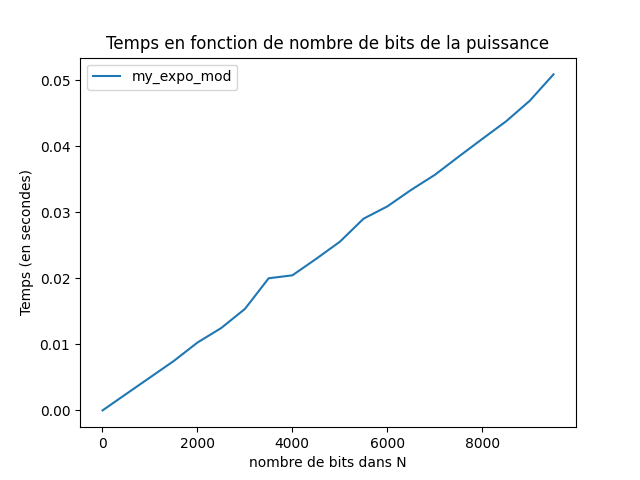
\includegraphics[width=0.7\linewidth]{Temps en fonction de nombre de bits de la puissance.png}
    \caption{}
    \label{fig:exp_mod}
\end{figure}

Avec cette courbe, on peut en déduire que my\_exp\_mod croit de manière lineaire au nombre de bits dans N.
(donc logaritmiquement par rapport à N)
\section{Nombres pseudo-premier de Carmichael}

\subsection{Méthode déterministe test primalité}

Ce teste sera une référence pour valider nos tests probabiliste
\begin{lstlisting}[language=Python, caption=Implementation test primalité naïf]
def first_test(N):
    """
    int -> boolean
    """
    for i in range(2, int(np.sqrt(N))+1):
        if(N%i == 0): return False
    return True
\end{lstlisting}

\subsubsection{Complexité}
Cet algorithme a une complexité en $\mathcal{O}(\sqrt{n})$ avec n le nombre testé.

\subsubsection{Temps d'exécution expérimenté}

\begin{figure}[H]
    \centering
    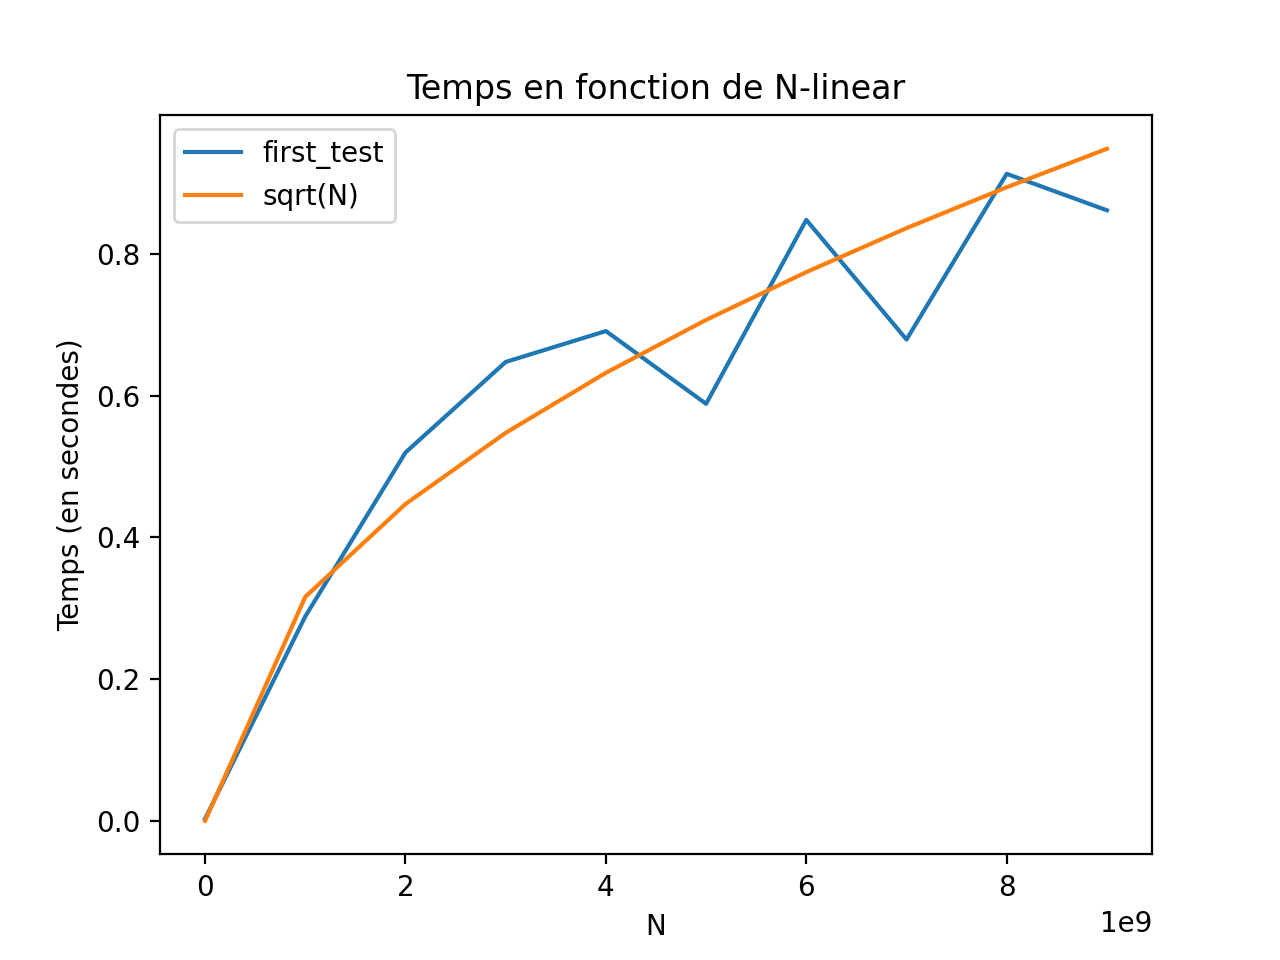
\includegraphics[width=0.7\linewidth]{first_test.png}
    \caption{}
    \label{fig:first_test}
\end{figure}

On voit bien sur la figure que la complexité expérimenté semble tendre vers la complexité $\mathcal{O}(\sqrt{n})$
où $n = 2^t$, la complexité est donc exponentielle en nombre de bits du nombre n, $\mathcal{O}(2^{t/2})$
\subsubsection{Nombre premier compté}
Cette fonctions permet de compter 9592 nombres premier jusqu'a $10^5$.

\subsection{isCarmichael}
Un nombre n est de carmichael, si n est un nombre composé, $\forall b<n, \mathit{PGCD}(b, n)=1 \implies b^{n-1} \equiv 1 [n]$
\begin{lstlisting}[language=Python, caption=Implementation test Carmichael]
def isCarmichael(n):
    n_divisors = 0
    for i in range(2, n):
        # (i premier avec n => i**(n-1) = 1[n])
        gcd = my_gcd(i, n)
        if (gcd == 1) and (my_expo_mod(i, n-1, n) != 1):
            return False

        if n%i == 0:
            n_divisors += 1

    if n_divisors == 0:
        # n est premier 
        return False
    
    return True
\end{lstlisting}

une implementation plus rapide est possible en utilisant le critère de korselt, conaissant les facteurs premiers du nombre, si n n'est pas divisible par un carré de premier, et quelque soit le facteur p de n, $(p-1) \equiv 0[n-1]$

\begin{lstlisting}[language=Python, caption=Implementation test Carmichael_korselt]
def isCarmichael_facteurs(n, facteurs):
    """
    int*list->boolean
    tester si n est un nombre de carmichael, etant donné ses facteurs
    """
    for facteur in facteurs:
        # pas facteur premier carré
        if(n%(facteur**2) == 0):
            return False
        if((n-1)%(facteur-1) != 0):
            return False
    # pass le test
    return True
\end{lstlisting}
% Cette fonction retourne vrai si n est un nombre de Carmichael, faux sinon.\\

Note: une fonction gen\_carmichael est aussi disponible, qui utilise cette fonction et boucle sur tout les entiers jusqu'à une limite et liste tout les nombres de Carmichael jusqu'à cette dernière.

\subsubsection{le nombre de nombres premiers inferieur à $10^5$}
En utilisant notre methode deterministe, on trouve : 9592 nombres premiers, ce qui fait un ratio de $\frac{9592}{10^{5}}$, soit $9.59\% $

\subsubsection{Nombres de Carmichael listé}
Voici la liste des nombres de Carmichael trouvé jusqu'à $10^5$ avec cette fonction : 561, 1105, 1729, 2465, 2821, 6601, 8911, 10585, 15841, 29341, 41041, 46657, 52633, 62745, 63973 et 75361.

\subsubsection{Plus grand nombre trouvé}
Avec cette méthode, le plus grand nombre de Carmichael trouvé en approximativement 5 minutes est 1909001.
(Note: une fonction experience\_carmichael\_t a été créé pour cette expérience.)

\section{Methodes probabiliste}
\subsection{gen\_carmichael3}

\begin{lstlisting}[language=Python, caption=gen\_carmichael3]
def gen_carmichael3(N=1e5, n_facteur_max=5):
    """
    int->int
    """
    premiers = [i for i in range(3, int(N), 2) if first_test(i)]
    nb_facteur = 3

    while True:
        acc = [premiers[np.random.randint(0, len(premiers)-1)]
                    for i in range(nb_facteur)]
        n = np.prod(acc, dtype=np.int64)

        if isCarmichael_facteurs(n, acc):
            return n
\end{lstlisting}

\subsubsection{Plus grand nombre trouvé}
Avec cette méthode, le plus grand nombre de Carmichael trouvé en approximativement 5 minutes est 3610008963601. (Ce résultat varie étant donné le coté aléatoire de gen\_carmichael3)
(Note: une fonction experience\_carmichael3\_t a été créé pour cette expérience.)

%Exercice 3 a partir d'ici

\subsection{Test\_fermat}

le test de fermat n'emmet pas de faux positifs, donc si test\_fermat retourne false, on est sure à 100\% qu'il s'agit d'un nombre composé, mais on ne peux savoir si elle retourne vrai et n sera donc possible premier avec une certaine probabilité.

Cette fonction prend n un entier impair,et retourne vrai si premier possible ou faux si composé de manière certaine.
\begin{lstlisting}[language=Python, caption=test\_fermat]
def test_fermat(n, a=None):
    """
    n un entier impair
    Retourne vrai si premier possible
    faux si composé
    """
    if a == None:
        a = random.randrange(2, n)
    return my_expo_mod(a, n-1, n) == 1
\end{lstlisting}


\subsubsection{Taux d'erreurs}
Note: Les pourcentage qui vont suivre sont fait sur $5 * 10^4$ valeurs de taille maximale $10^5$ et les nombre tiré aléatoirement sont tous impaire.\\

\begin{figure}[H]
\begin{subfigure}{.5\linewidth}
\centering
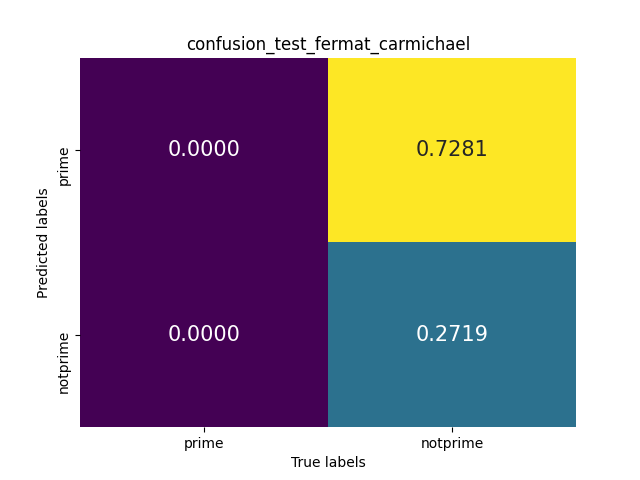
\includegraphics[scale=0.45]{confusion_test_fermat_carmichael.png}
\caption{\centering confusion fermat avec nombre de carmichael}
\label{fig:sub1}
\end{subfigure}%
\begin{subfigure}{.5\linewidth}
\centering
\includegraphics[scale=0.45]{confusion_test_fermat_aleatoire composé.png}
\caption{\centering confusion fermat avec nombre aleatoire composé}
\label{fig:sub2}
\end{subfigure}\\[1ex]
\begin{subfigure}{\linewidth}
\centering
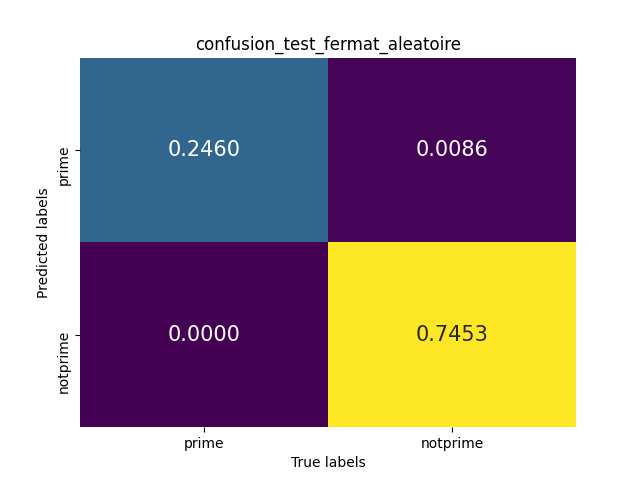
\includegraphics[scale=0.45]{confusion_test_fermat_aleatoire.png}
\caption{\centering confusion fermat avec nombre aleatoire}
\label{fig:sub3}
\end{subfigure}
\caption{\centering Matrice de confusion test fermat}
\label{fig:test}
\end{figure}


En tirant seulement des nombres de Carmichael, on obtient un taux d'erreur d'environ 72.81\%.\\
En tirant seulement des nombres composé aléatoire, on obtient un taux d'erreur d'environ 1.22\%.\\
En tirant des nombres aléatoires, on obtient un taux d'erreur d'environ 0.8\%.\\

nous pouvons voir clairement que fermat n'emmet jamais des faux negatifs, et toutes nos erreur sont des faux positifs, de cette nature on ne peut utiliser un teste de fermat dans des cas concret pour assurer la primalité d'un nombre, par contre il pourrait servir dans une co-routine pour éliminer rapidement des nombres qui ne sont pas premier, et reduire l'espace de recherche pour utiliser d'autre testes plus precis.

\subsection{test\_miller\_rabin}

Dans cette partie nous allons coder un algorithme plus robuste que le teste de fermat .\\[1.5cm]


\begin{lstlisting}[language=Python, caption=Implementation test\_miller\_rabin]
def test_miller_rabin(n, T=10):
    """
    int*int->boolean
    n = 1 + 2**h * m
    """

    p_h = 1
    temp = n-1
    while(temp%2 == 0):
        temp = temp // 2
        p_h *= 2
    m = (n-1)//p_h

    inf = n-3
    for i in range(T):
        a = 2 + random.getrandbits(n.bit_length())%(n-3)
        b = my_expo_mod(a, m, n)

        if b==1 or b==(n-1):
            continue

        for j in range(1, p_h):
            if b!=(n-1) and my_expo_mod(b, 2, n)==1:
                return False
            elif  b==(n-1):
                break
            b = my_expo_mod(b, 2, n)
        
        if b != (n-1):
            return False
    
    return True
\end{lstlisting}

\subsection{Taux d'erreur}


\begin{figure}[H]
\begin{subfigure}{.5\linewidth}
\centering
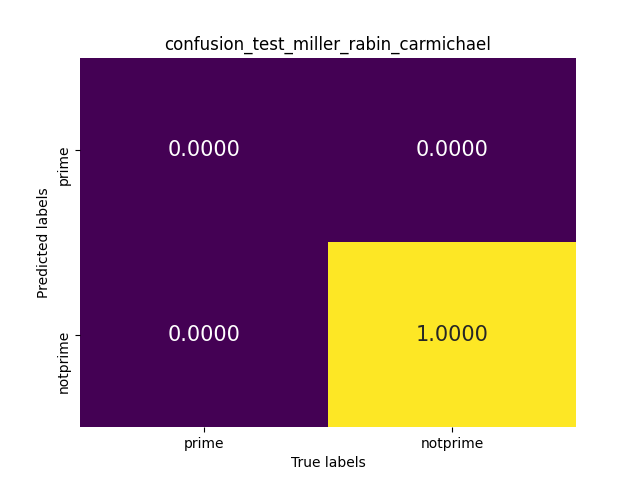
\includegraphics[scale=0.45]{confusion_test_miller_rabin_carmichael.png}
\caption{\centering confusion miller rabin avec nombre de carmichael}
\label{fig:sub1}
\end{subfigure}%
\begin{subfigure}{.5\linewidth}
\centering
\includegraphics[scale=0.45]{confusion_test_miller_rabin_aleatoire composé.png}
\caption{\centering confusion miller rabin avec nombre aleatoire composé}
\label{fig:sub2}
\end{subfigure}\\
\begin{subfigure}{\linewidth}
\centering
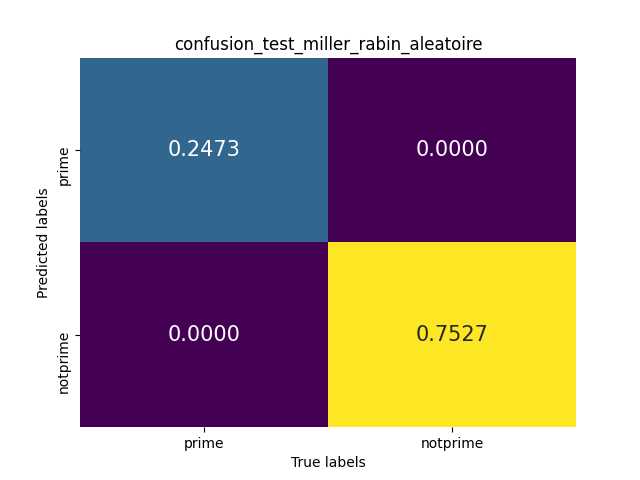
\includegraphics[scale=0.45]{confusion_test_miller_rabin_aleatoire.png}
\caption{\centering confusion miller rabin avec nombre aleatoire}
\label{fig:sub3}
\end{subfigure}
\caption{\centering Matrice de confusion test miller rabin}
\label{fig:test}
\end{figure}

En tirant seulement des nombres de Carmichael, on obtient un taux d'erreur 0\%.\\
En tirant seulement des nombres composé aléatoire, on obtient un taux d'erreur d'environ 0\%.\\
En tirant des nombres aléatoires, on obtient un taux d'erreur d'environ 0\%.\\

Pour avoir plus d'informations, nous testons l'effet du nombre d'experiences sur la probabilité d'erreur de miller rabin


 \begin{figure}[H]
    \centering
     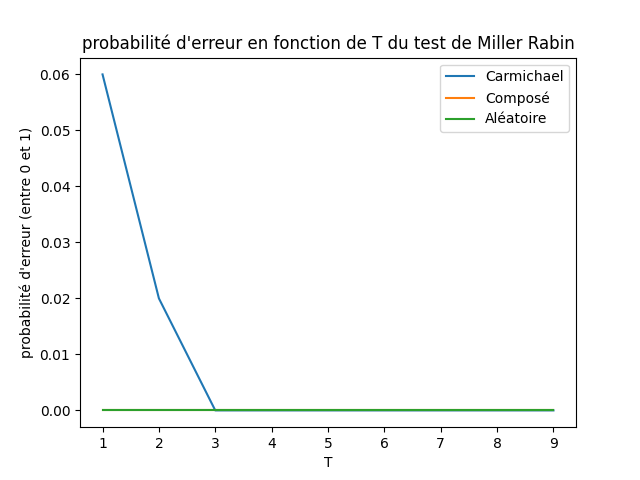
\includegraphics[scale=0.4]{miller_rabin_test_T.png}
     \caption{\centering Effet de T(nbr d'experiences) sur probabilité erreur miller\_rabin}
 \end{figure}

% \subsection{comparaison temps d'execution, miller\_rabin vs fermat}
%  \begin{figure}[H]
%     \centering
%      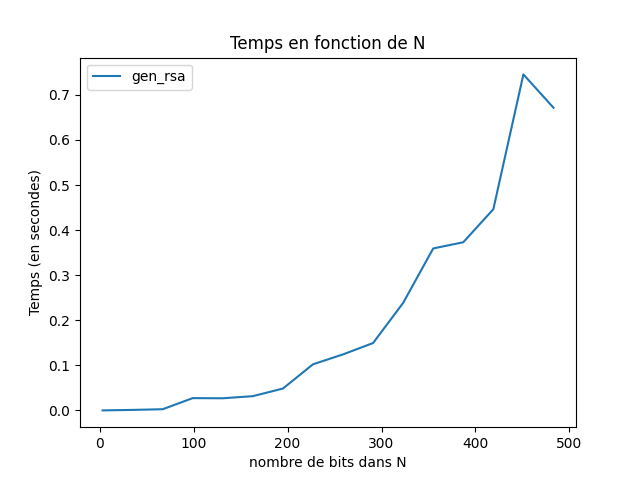
\includegraphics[scale=0.6]{Temps en fonction de N.png}
%      \caption{\centering temps d'execution de gen_rsa}
%  \end{figure}
 
\subsection{RSA}

\subsubsection{gen\_rsa}

\begin{lstlisting}[language=Python, caption=gen\_rsa]
def gen_rsa(t):
    """
    int: longeur en bits (doit être supérieur a 2)
    return: (e, n), (d, n)
    """

    inf = 1<<(t-1)

    while True:
        p = inf + random.getrandbits(t-1)
        if test_miller_rabin(p):
            break
    while True:
        q = inf + random.getrandbits(t-1)
        if test_miller_rabin(q) and q != p:
            break

    return p, q, p*q
\end{lstlisting}

\subsection{Temps d'execution}
gen\_rsa est exponentiel en nombres de bits
 \begin{figure}[H]
    \centering
     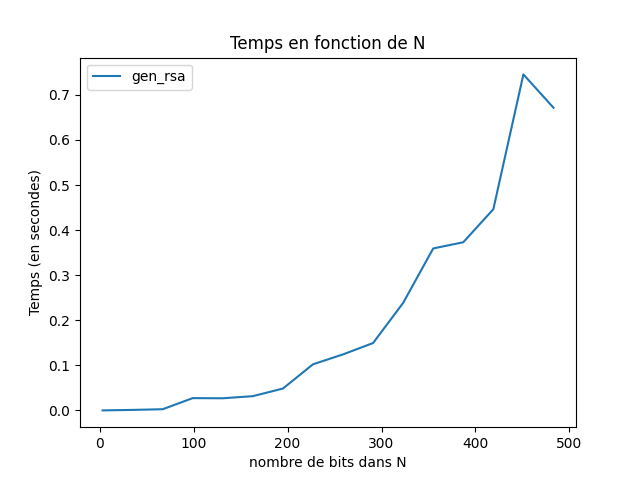
\includegraphics[scale=0.6]{Temps en fonction de N.png}
     \caption{\centering temps d'execution de gen\_rsa par rapport à la taille des nombres en bits}
 \end{figure}

\newpage
\subsubsection{BONUS:}

%nous n'avons pas voulu laisser les choses à moitié fini 

Il aurait été dommage de conclure sans terminer le protocole RSA, nous avons donc aussi implémenté une fonction RSA, générant une paire de clef privée et public.
Ces dernières sont utilisable dans les dernières fonctions, encode et decode pour encoder et décoder des messages.

On commence d'abords par générer 2 nombres premiers grands $p, q$ , pour construire un nombre $n = p.q$
$\phi(n)$ est le nombre de nombres premier avec n (ce qui est dure a calculer directement), alors on chercherait plutôt à utiliser l'inverse n - nombre\_pas\_premier\_avec\_n, qui est beaucoup plus facile étant donné qu'on connaît les seuls diviseur de n (p et q), et donc un nombre pas premier avec n s'écrirait 
\begin{equation} \label{eq1}
\begin{split}
\mathit{nombre\_pas\_premier\_avec\_n} & = \# (\{i.p\ | i \in [1 \dots q]\}\cup \{i.q\ | i \in [1 \dots p]\})\\
 & = (q-1) + (p-1) + 1 \\
 & = (q-1) + p
\end{split}
\end{equation}
 
\begin{equation} \label{eq1}
\begin{split}
\phi(n) & = n - \mathit{nombre\_pas\_premier\_avec\_n} \\
 & = p.q - ((q-1) + p) \\
 & = p.q - (q-1) - p \\
 & = p(q-1) - (q-1) \\
 & = (q-1).(p-1)
\end{split}
\end{equation}
 l'etape suivant consiste à trouve un nombre inversible modulo $\phi(n)$ $e, d$ 
 $$d.e \equiv 1[\phi(n)]$$

 ces deux nombre $e, d$, constitueront ,avec n, respectivement la clé\_publique, et la clé\_privé\\[1cm]
 
\begin{lstlisting}[language=Python, caption=RSA]
def RSA(t):
    """
    return public_key, private_key
    """
    p, q, n = gen_rsa(t)

    # phi (nombre de nombres premier avec n, < n)
    phi = (p-1)*(q-1)

    while True:
        e = 2 + random.getrandbits(phi.bit_length())%(phi-3)
        gcd, _, d = my_gcd_etendu(phi, e)
        if(gcd == 1):
            break
    
    return (e, n), (d, n)
\end{lstlisting}


Pour encoder un message $m$ il suffit de faire $s = m^e[n]$ et finallement pour décoder $m = s^d[n]$
cela marche en utilisant le petit theorem de fermat ameliotré: 
$$a^{\phi(n)} \equiv 1 [n]$$
$$s^d = (m^e)^d = m^{e.d} = m^{1 + k.\phi(n)} = m^1.m^{\phi(n) = m[n]}$$ 

\begin{lstlisting}[language=Python, caption=Encodage et décodage]
def encode(m, public_key):
    """
    (e, n)
    """
    return [my_expo_mod(ord(c), *public_key) for c in m]

def decode(m, private_key):
    """
    (d, n)
    """
    return ''.join([chr(my_expo_mod(c, *private_key)) for c in m])
\end{lstlisting}


% Summary and Conclusions

\section{Conclusions}

Pour conclure

%Dans ce projet, nous avons pu découvrir plus en profondeur le problème de primalité.
A travers ces différents exercices, nous avons implémenté plusieurs algorithmes probabilistes dans le but de répondre au problème de la primalité. Au vu des résultat obtenue, nous nous somme rendu compte de l'intérêt et de la puissance des algorithme probabiliste, qui dans ce cas ci, permettent de répondre au problème de primalité avec des taux d'erreur très acceptable et des vitesses supérieur aux algorithmes déterministes classique.
L'utilité de ce type d'algorithme est d'autant plus concrète une fois appliqué sur des problèmes plus concrets tel que le chiffrement RSA par exemple, nous obtenons une vitesse de chiffrement très convenable, chose qui n'aurait pas été possible en utilisant le test de primalité classique.
    

\end{document}
